TODO Explain that we mostly aim replicate previous work in terms of experiments (we don't expect accuracy improvements)

\subsection{Datasets}

It is interesting to see how non-parametric models perform on various types of
inputs. Goldwater et. al show the model accuracy and convergeence on English
words. While comparing our models' performace on English with Goldwater et. al,
we also want to look at how the models generalize to languages with similar
morphology. We run the baseline and our models on English verbs (EN-PTB) (the
dataset used in \cite{goldwater2011}) and Russian adjectives (RU-ADJ). The
EN-PTB words are extracted from the Penn Treebank and the RU-ADJ words are from
the Russian national corpus.

The following sections gives a brief overview of the morphology of Ebglish
verbs and Russian adjectives and why they suit the models we are using in this
work.  

\subsubsection{English verbs}

English verbs inflect is very straight forward. Words can be seen as a
combination of a single prefix and a suffix, unlike more morephologically
languages where many morphemes can join to form words. There are mainly three
classes of suffixes that words can take apart from the empty suffix.

\begin{table}[h]
\centering
\begin{tabular}{lll}
\hline
\multicolumn{3}{c}{\textbf{Regular Inflections}} \\
\hline
Morpheme & Description & Examples \\
\hline
-s, -es & occurs wih 3rd person singular & walk-s, run-s, camp-s \\
-ed & past marker & work-ed, bark-ed, camp-ed \\
-n & past participle marker & chose-n, prove-n, woke-n \\
-ing & present participle marker & bark-ing, work-ing, camp-ing \\
\hline
\multicolumn{3}{c}{\textbf{Irregular Inflections}} \\
\hline
\textit{unclear} & past marker & ran, ate \\
\textit{unclear} & past participle marker & drunk, hung \\
\hline
\end{tabular}
\caption{\label{enInflections}Regular and irregular inflections for English verbs}
\end{table}



\subsubsection{Russian adjectives}


\begin{table}[h]
\centering
\begin{tabular}{lcc}
\hline
Dataset & Types & Tokens \\
\hline
EN-PTB & 7K & 113K \\
RU-ADJ & 9K & 18K \\
\hline
\end{tabular}
\caption{Types and Tokens in the datasets}
\label{datastats}
\end{table}

Table~\ref{datastats} gives the types and tokens in the datasets.

\begin{figure}[ht]
\begin{minipage}[b]{0.45\linewidth}
\centering
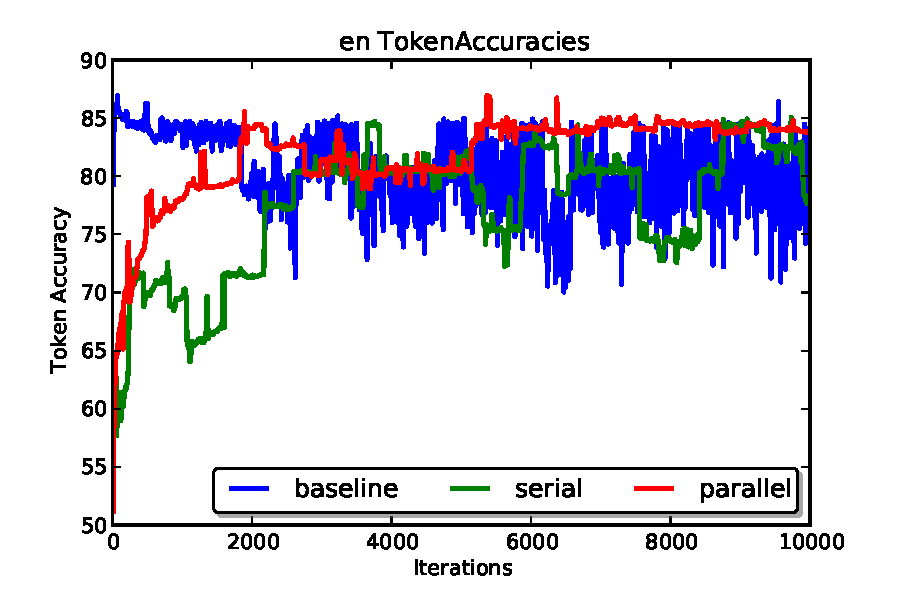
\includegraphics[width=\textwidth]{fig/en_TokenAccuracies}
\end{minipage}
\hspace{0.5cm}
\begin{minipage}[b]{0.45\linewidth}
\centering
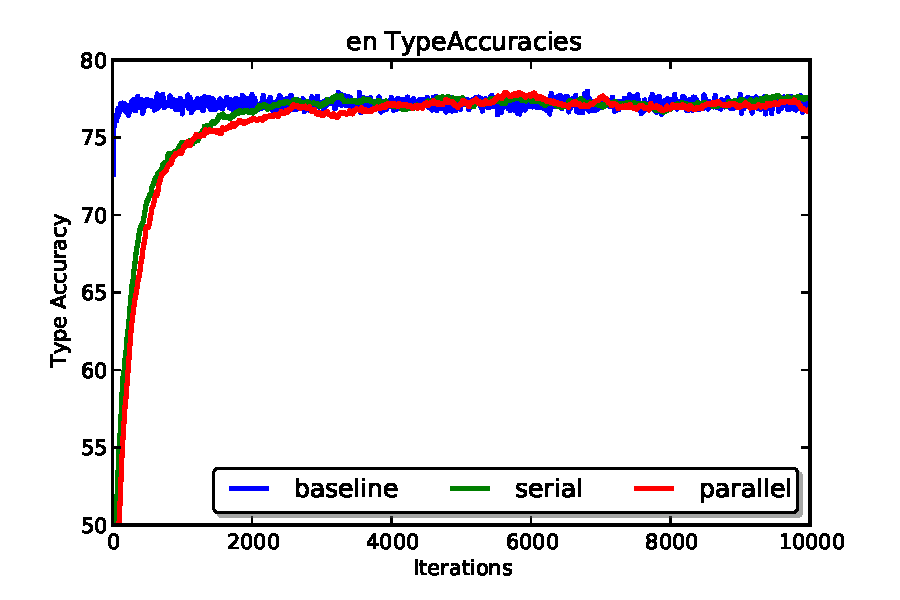
\includegraphics[width=\textwidth]{fig/en_TypeAccuracies}
\end{minipage}
\caption{\label{fig:enacc}Token and Type Accuracies for English verbs over 10K iterations}
\end{figure}

\begin{figure}[ht]
\begin{minipage}[b]{0.45\linewidth}
\centering
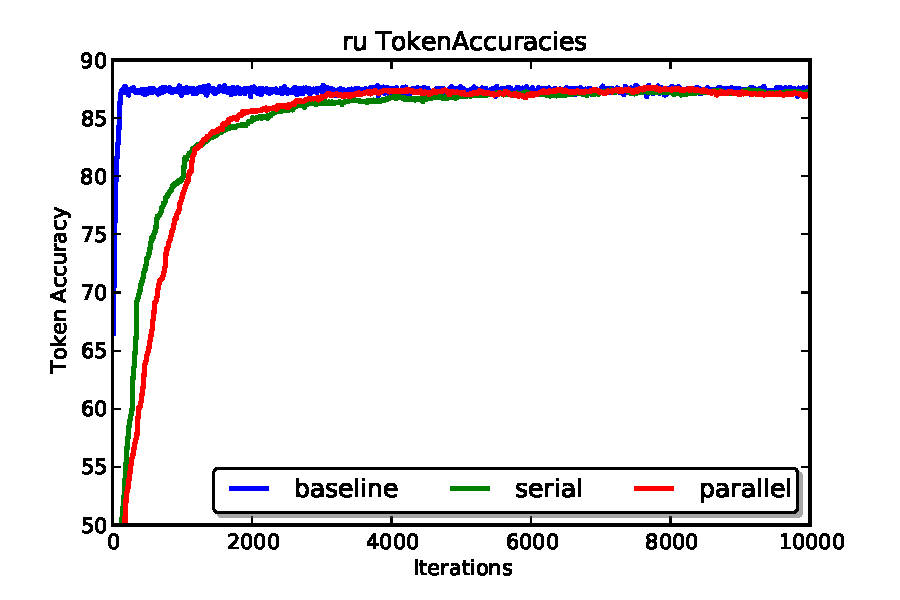
\includegraphics[width=\textwidth]{fig/ru_TokenAccuracies}
\end{minipage}
\hspace{0.5cm}
\begin{minipage}[b]{0.45\linewidth}
\centering
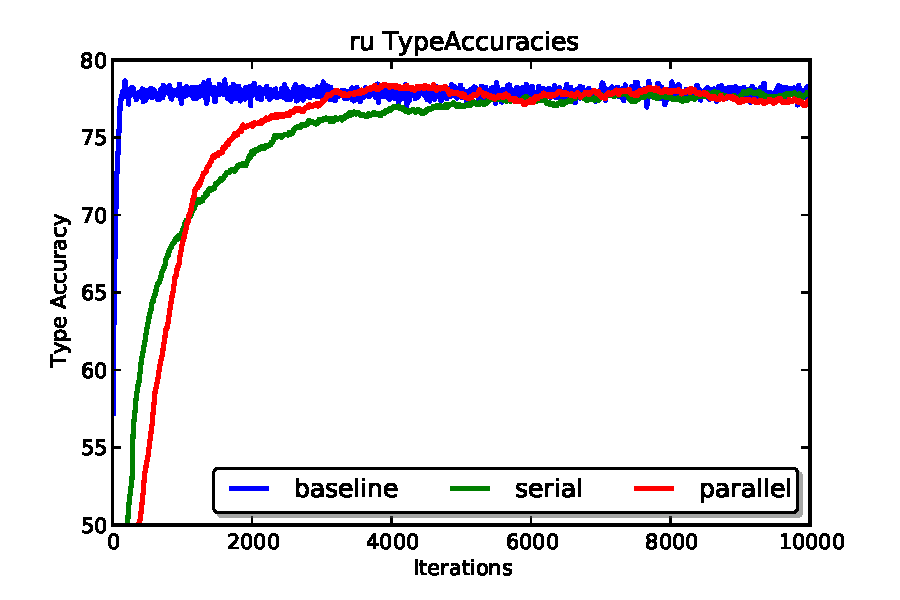
\includegraphics[width=\textwidth]{fig/ru_TypeAccuracies}
\end{minipage}
\caption{\label{fig:ruacc}Token and Type Accuracies for Russian adjectives over 110K iterations}
\end{figure}


\begin{figure}[ht]
\begin{minipage}[b]{0.45\linewidth}
\centering
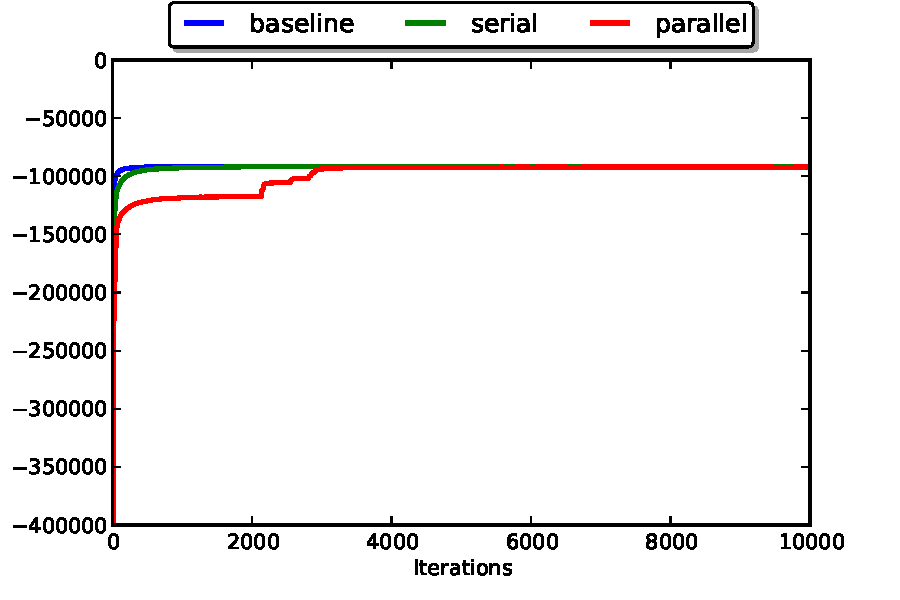
\includegraphics[width=\textwidth]{fig/en_base_lls}
\end{minipage}
\hspace{0.5cm}
\begin{minipage}[b]{0.45\linewidth}
\centering
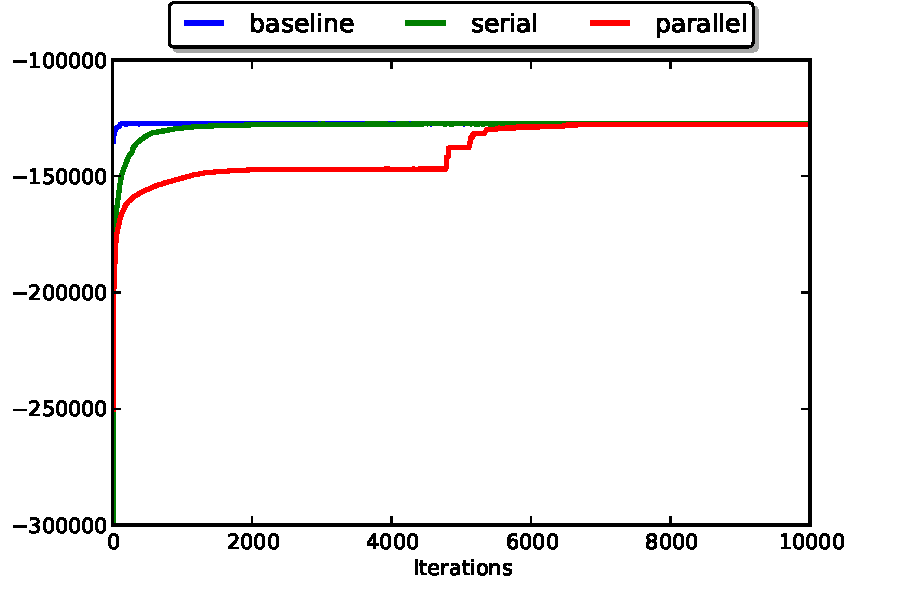
\includegraphics[width=\textwidth]{fig/ru_base_lls}
\end{minipage}
\caption{\label{fig:basell} Base log-likelihood for all the three models}
\end{figure}

\begin{figure}[ht]
\begin{minipage}[b]{0.45\linewidth}
\centering
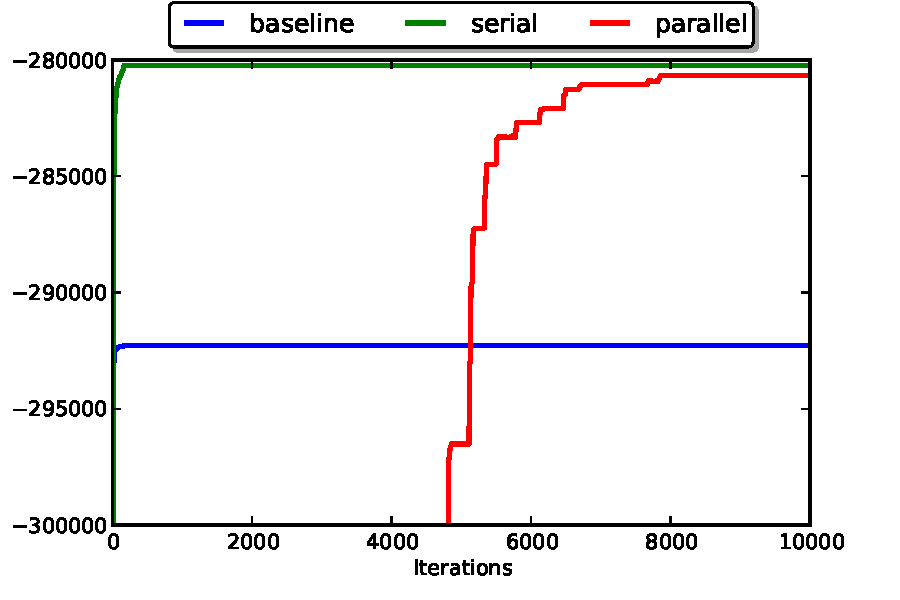
\includegraphics[width=\textwidth]{fig/ru_crp_lls}
\end{minipage}
\hspace{0.5cm}
\begin{minipage}[b]{0.45\linewidth}
\centering
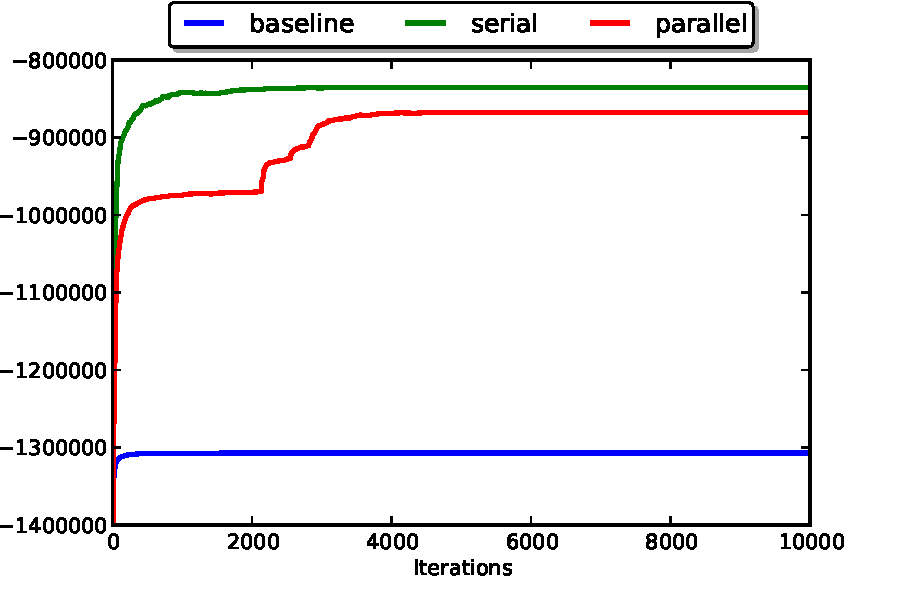
\includegraphics[width=\textwidth]{fig/en_crp_lls}
\end{minipage}
\caption{\label{fig:crpll} CRP log-likelihood for all the three models}
\end{figure}


\begin{figure}[ht]
\begin{minipage}[b]{0.45\linewidth}
\centering
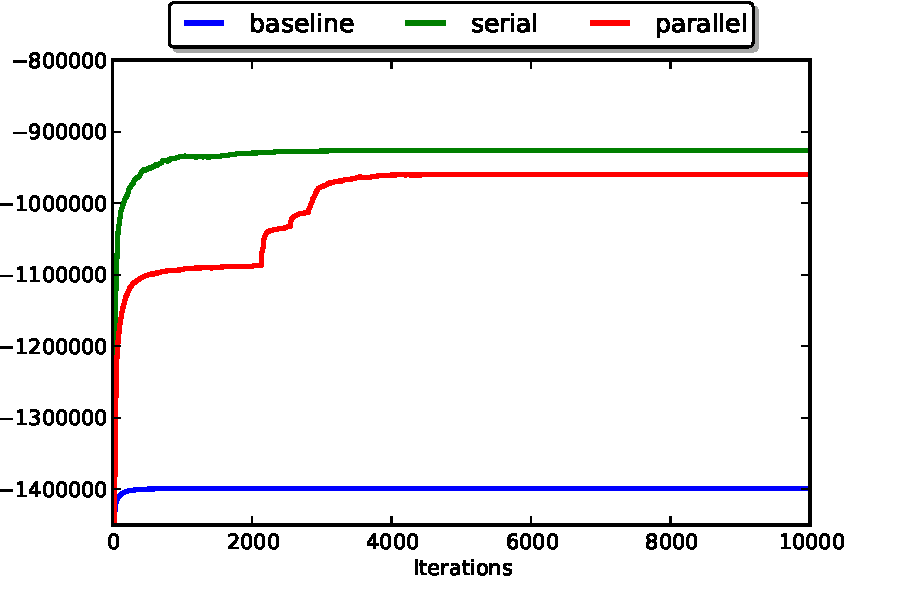
\includegraphics[width=\textwidth]{fig/en_lls}
\end{minipage}
\hspace{0.5cm}
\begin{minipage}[b]{0.45\linewidth}
\centering
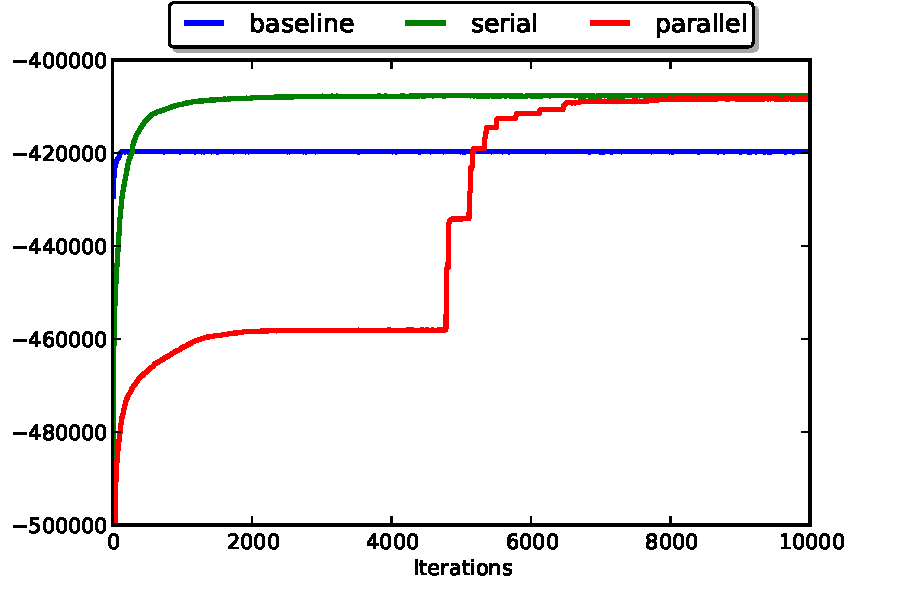
\includegraphics[width=\textwidth]{fig/ru_lls}
\end{minipage}
\caption{\label{fig:ll} Complete log-likelihood for all the three models}
\end{figure}

